\chapter{Methodology}

\begin{figure}[htp]
    \centering
    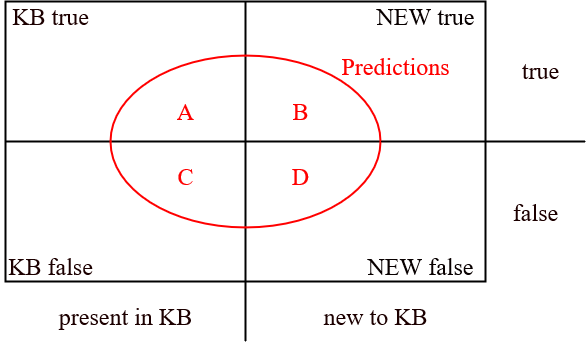
\includegraphics[width=10cm]{figures/kb_venn.png}
    \caption{KB prediction under incompleteness}
\end{figure}

\begin{figure}[htp]
    \centering
    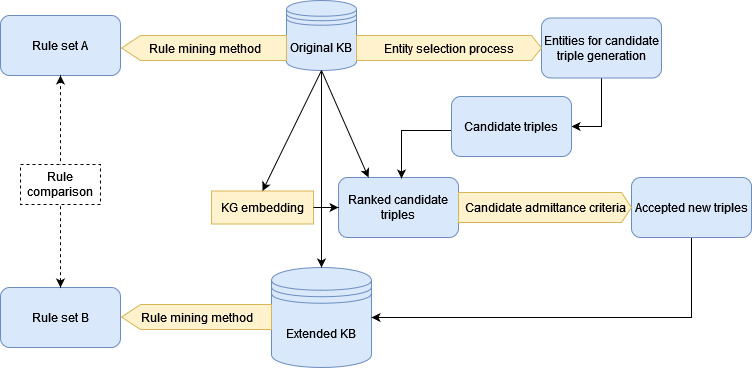
\includegraphics[width=12cm]{figures/ontology_mining_pipeline.jpg}
    \caption{KB prediction under incompleteness}
\end{figure}


\section{KB generation}
While there are many large KBs publicly available, they are often quite complex in the number of different relations and entities used. Since we are mining rules over relations, the relational aspect of the KBs used was kept simple. By limiting the number of relations used in the KBs the resulting rules mined won't be overly diverse, and therefore easier for a human to understand evaluate. Two different datasets were used to conduct the experiments, both of which had been limited to contain only six different types of relations.


\subsection{Wikidata5M - family subset}
Wikidata5M is a knowledge-graph dataset containing over 20 million triples. It combines information from the Wikidata KG with Wikipedia pages \cite{wang2019kepler}. Wikidata5M uses the same identifier system as Wikidata, where each entity and relation is assigned a unique ID. The IDs of entities are prefixed with \texttt{Q} and those of relations with \texttt{P}. For example the following line \\
\centerline{\texttt{\href{https://www.wikidata.org/wiki/Q146}{Q146} \quad \href{https://www.wikidata.org/wiki/Property:P279}{P279} \quad  \href{https://www.wikidata.org/wiki/Q39201}{Q39201}}} \
corresponds to \textless\texttt{\href{https://www.wikidata.org/wiki/Q146}{house cat}, \href{https://www.wikidata.org/wiki/Property:P279}{subclass of}, \href{https://www.wikidata.org/wiki/Q39201}{pet}}\textgreater, where each entity has a corresponding Wikipedia page.
This dataset was chosen due to its size and because it contained an easily comprehendable relational subset, namely relations concerning family structure. 
\begin{lstlisting}[language=Python, caption={Python dictionary converting family predicate IDs to their names},captionpos=t, label={family_predicated_dict}]
family_predicates_dict = {
    'P40': 'child', 
    'P22' : 'father', 
    'P25' : 'mother',
    'P26' : 'spouse', 
    'P1038' : 'relative', 
    'P3373' : 'sibling', 
}
\end{lstlisting}

After filtering out all triples that did not use one of the six selected family predicates, the IDs were converted to meaningful names so that the resulting rules mined would be easily readable. The python dictionary listen in \ref{family_predicated_dict} shows the chosen predicates. A few other family predicates were considered, but did not have as many corresponding data points or were too similar to other selected predicates. Predicates such as \texttt{grandchild} or \texttt{sister} are also not currently used in Wikidata, and from a discussion in the Wikidata community it seems that all properties considered redundant were removed \cite{kinship_discussion}. For the experiments Pykeen's distribution of the dataset was used \cite{ali2021pykeen}. The resulting Wikidata KB contained around 250 000 triples.

\subsection{WN18RR}

\section{Model selection}


\section{Candidate generation and ranking}



\section{Rule mining and evaluation}
